% Options for packages loaded elsewhere
\PassOptionsToPackage{unicode}{hyperref}
\PassOptionsToPackage{hyphens}{url}
\PassOptionsToPackage{dvipsnames,svgnames,x11names}{xcolor}
%
\documentclass[12pt, oneside]{report}

% Inputs the Document Packages
\usepackage{array}
\usepackage{blindtext}
\usepackage[
    citestyle=verbose-ibid,
    bibstyle=authoryear,
    autocite=footnote,
    notetype=endonly,
    backend=biber,
    isbn=false, 
    doi=false,
    labeldateparts
]{biblatex}
\usepackage{booktabs}
\usepackage{ctable}
\usepackage{fancyhdr}
\usepackage{graphicx}
\usepackage{hyperref}
%\usepackage[hidelinks]{hyperref}
\usepackage[utf8]{inputenc}
\usepackage{mobilizing-justice}
\usepackage{multicol}
\usepackage{pdfpages}
% Change font size
\usepackage{relsize}
\usepackage{setspace}
\usepackage{subfig}
\usepackage{tcolorbox}
\tcbuselibrary{theorems}
\usepackage{wrapfig}


% Pointing to a bib resource here
\addbibresource[label=main]{bibliography.bib} % REPLACE WITH WORKS CITED BIB FILE

% Remove URL and DOI for cleaner citations (optional, obviously)
\AtEveryBibitem{
    \clearfield{url}
    \clearfield{doi}
}

\let\oldheadrule\headrule% Copy \headrule into \oldheadrule
\renewcommand{\headrule}{\color{Maroon}\oldheadrule}% Add colour to \headrule
\renewcommand{\headrulewidth}{12.5pt}

% HERE GOES THE TITLE FOR THE DOCUMENT
  \title{Accessibility analysis for planning applications}


\usepackage{amsmath,amssymb}
\usepackage{iftex}
\ifPDFTeX
  \usepackage[T1]{fontenc}
  \usepackage[utf8]{inputenc}
  \usepackage{textcomp} % provide euro and other symbols
\else % if luatex or xetex
  \usepackage{unicode-math}
  \defaultfontfeatures{Scale=MatchLowercase}
  \defaultfontfeatures[\rmfamily]{Ligatures=TeX,Scale=1}
\fi
\usepackage{lmodern}
\ifPDFTeX\else  
    % xetex/luatex font selection
\fi
% Use upquote if available, for straight quotes in verbatim environments
\IfFileExists{upquote.sty}{\usepackage{upquote}}{}
\IfFileExists{microtype.sty}{% use microtype if available
  \usepackage[]{microtype}
  \UseMicrotypeSet[protrusion]{basicmath} % disable protrusion for tt fonts
}{}
\makeatletter
\@ifundefined{KOMAClassName}{% if non-KOMA class
  \IfFileExists{parskip.sty}{%
    \usepackage{parskip}
  }{% else
    \setlength{\parindent}{0pt}
    \setlength{\parskip}{6pt plus 2pt minus 1pt}}
}{% if KOMA class
  \KOMAoptions{parskip=half}}
\makeatother
\usepackage{xcolor}
\setlength{\emergencystretch}{3em} % prevent overfull lines
\setcounter{secnumdepth}{-\maxdimen} % remove section numbering
% Make \paragraph and \subparagraph free-standing
\ifx\paragraph\undefined\else
  \let\oldparagraph\paragraph
  \renewcommand{\paragraph}[1]{\oldparagraph{#1}\mbox{}}
\fi
\ifx\subparagraph\undefined\else
  \let\oldsubparagraph\subparagraph
  \renewcommand{\subparagraph}[1]{\oldsubparagraph{#1}\mbox{}}
\fi


\providecommand{\tightlist}{%
  \setlength{\itemsep}{0pt}\setlength{\parskip}{0pt}}\usepackage{longtable,booktabs,array}
\usepackage{calc} % for calculating minipage widths
% Correct order of tables after \paragraph or \subparagraph
\usepackage{etoolbox}
\makeatletter
\patchcmd\longtable{\par}{\if@noskipsec\mbox{}\fi\par}{}{}
\makeatother
% Allow footnotes in longtable head/foot
\IfFileExists{footnotehyper.sty}{\usepackage{footnotehyper}}{\usepackage{footnote}}
\makesavenoteenv{longtable}
\usepackage{graphicx}
\makeatletter
\def\maxwidth{\ifdim\Gin@nat@width>\linewidth\linewidth\else\Gin@nat@width\fi}
\def\maxheight{\ifdim\Gin@nat@height>\textheight\textheight\else\Gin@nat@height\fi}
\makeatother
% Scale images if necessary, so that they will not overflow the page
% margins by default, and it is still possible to overwrite the defaults
% using explicit options in \includegraphics[width, height, ...]{}
\setkeys{Gin}{width=\maxwidth,height=\maxheight,keepaspectratio}
% Set default figure placement to htbp
\makeatletter
\def\fps@figure{htbp}
\makeatother
\newlength{\cslhangindent}
\setlength{\cslhangindent}{1.5em}
\newlength{\csllabelwidth}
\setlength{\csllabelwidth}{3em}
\newlength{\cslentryspacingunit} % times entry-spacing
\setlength{\cslentryspacingunit}{\parskip}
\newenvironment{CSLReferences}[2] % #1 hanging-ident, #2 entry spacing
 {% don't indent paragraphs
  \setlength{\parindent}{0pt}
  % turn on hanging indent if param 1 is 1
  \ifodd #1
  \let\oldpar\par
  \def\par{\hangindent=\cslhangindent\oldpar}
  \fi
  % set entry spacing
  \setlength{\parskip}{#2\cslentryspacingunit}
 }%
 {}
\usepackage{calc}
\newcommand{\CSLBlock}[1]{#1\hfill\break}
\newcommand{\CSLLeftMargin}[1]{\parbox[t]{\csllabelwidth}{#1}}
\newcommand{\CSLRightInline}[1]{\parbox[t]{\linewidth - \csllabelwidth}{#1}\break}
\newcommand{\CSLIndent}[1]{\hspace{\cslhangindent}#1}

% TODO: Add custom LaTeX header directives here

\usepackage{xstring} 

\usepackage[none]{hyphenat} %removes the hyphenation across lines for the justified setting.

\newcommand*{\ExtractFirstChar}[1]{%
    %% #1 = string to extract first char from
    %\fullexpandarg
    %\IfBeginWith{#1}{\{}{%
    %    \StrChar{#1}{2}[\FirstChar]%
    %}{%
        \StrChar{#1}{1}[\FirstChar]%
    %}%
    \FirstChar
}
\makeatletter
\makeatother
\makeatletter
\makeatother
\makeatletter
\@ifpackageloaded{caption}{}{\usepackage{caption}}
\AtBeginDocument{%
\ifdefined\contentsname
  \renewcommand*\contentsname{Table of contents}
\else
  \newcommand\contentsname{Table of contents}
\fi
\ifdefined\listfigurename
  \renewcommand*\listfigurename{List of Figures}
\else
  \newcommand\listfigurename{List of Figures}
\fi
\ifdefined\listtablename
  \renewcommand*\listtablename{List of Tables}
\else
  \newcommand\listtablename{List of Tables}
\fi
\ifdefined\figurename
  \renewcommand*\figurename{Figure}
\else
  \newcommand\figurename{Figure}
\fi
\ifdefined\tablename
  \renewcommand*\tablename{Table}
\else
  \newcommand\tablename{Table}
\fi
}
\@ifpackageloaded{float}{}{\usepackage{float}}
\floatstyle{ruled}
\@ifundefined{c@chapter}{\newfloat{codelisting}{h}{lop}}{\newfloat{codelisting}{h}{lop}[chapter]}
\floatname{codelisting}{Listing}
\newcommand*\listoflistings{\listof{codelisting}{List of Listings}}
\makeatother
\makeatletter
\@ifpackageloaded{caption}{}{\usepackage{caption}}
\@ifpackageloaded{subcaption}{}{\usepackage{subcaption}}
\makeatother
\makeatletter
\@ifpackageloaded{tcolorbox}{}{\usepackage[skins,breakable]{tcolorbox}}
\makeatother
\makeatletter
\@ifundefined{shadecolor}{\definecolor{shadecolor}{rgb}{.97, .97, .97}}
\makeatother
\makeatletter
\makeatother
\makeatletter
\makeatother
\ifLuaTeX
  \usepackage{selnolig}  % disable illegal ligatures
\fi
\IfFileExists{bookmark.sty}{\usepackage{bookmark}}{\usepackage{hyperref}}
\IfFileExists{xurl.sty}{\usepackage{xurl}}{} % add URL line breaks if available
\urlstyle{same} % disable monospaced font for URLs
\hypersetup{
  pdftitle={Accessibility analysis for planning applications},
  colorlinks=true,
  linkcolor={blue},
  filecolor={Maroon},
  citecolor={Blue},
  urlcolor={Blue},
  pdfcreator={LaTeX via pandoc}}

\title{Accessibility analysis for planning applications}
\usepackage{etoolbox}
\makeatletter
\providecommand{\subtitle}[1]{% add subtitle to \maketitle
  \apptocmd{\@title}{\par {\large #1 \par}}{}{}
}
\makeatother
\subtitle{Accessibility analysis for planning applications}
\author{Anastasia Soukhov \and Antonio Páez}
\date{2024-01-02}

\begin{document}
%-----------------------------------------------------------------------------%
%                            Set Page STYLE                                   %
%-----------------------------------------------------------------------------%

% THIS IS THE DEFAULT PAGE STYLE
\pagestyle{fancy}
\fancyhf{}
\renewcommand{\footrulewidth}{0pt}
\fancyfoot[R]{\textbf{\thepage}}
\fancyfoot[L]{Accessibility analysis for planning applications}
\renewcommand{\footrulewidth}{1pt}

% THE TABLE OF CONTENTS PAGE USES THIS STYLE
\fancypagestyle{plain}{%
  \renewcommand{\headrulewidth}{0pt}%
  \fancyhf{}%
  \renewcommand{\footrulewidth}{1pt}
  \fancyfoot[R]{\textbf{\thepage}}%
  % THE TITLE IS NOT ACTUALLY GOING HERE WHY??
  \fancyfoot[L]{Accessibility analysis for planning
applications} % HERE GOES THE TITLE
}

% IT IS ALSO POSSIBLE TO USE STYLE empty AS IN THE TITLE PAGE AND FINAL PAGE

%-----------------------------------------------------------------------------%
% START OF TITLE PAGE
%-----------------------------------------------------------------------------%
\thispagestyle{empty}

% Define a dimension for the height of the banner for the title page
\newdimen\bannerheight

% Set \bannerheight to the height of the banner
\settoheight{\bannerheight}{%
  
\includegraphics[width=\paperwidth]{images/title-banner.png}%
}

% Title banner top
\AddToShipoutPictureBG*{%
 \AtPageUpperLeft{\raisebox{-\height}{
\includegraphics[width=\paperwidth]{images/title-banner.png}}}
 }

% Cover picture
\AddToShipoutPictureBG*{%
 %\AtPageLowerLeft{\raisebox{0.5\height}{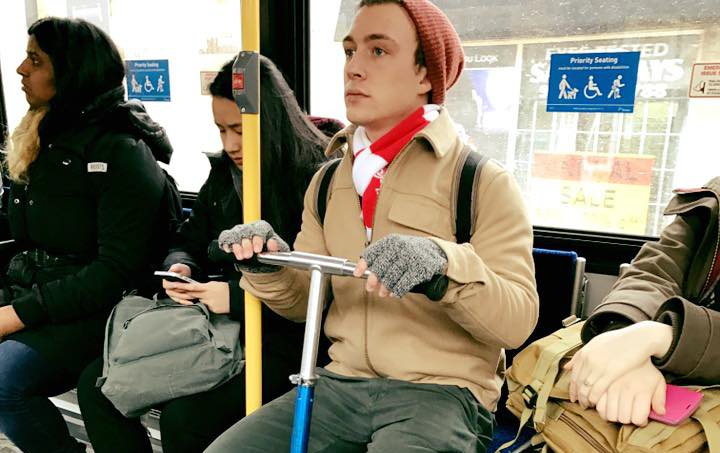
\includegraphics[width=\paperwidth]{images/cover-picture.png}}}
 \AtPageUpperLeft{\raisebox{-\bannerheight-\height}{
\includegraphics[width=\paperwidth]{images/potential-access-cover-image.jpeg}}}
 }

% HERE GOES THE TITLE OF THE DOCUMENT
  \vspace{-5cm}{\relscale{1.75}{\textcolor{white}{Accessibility analysis
for planning applications}}}\par%
% HERE GOES THE DOCUMENT TYPE; CURRENTLY HARDCODED BUT COULD BE AN INPUT IN template.qmd
{\relscale{1.25}{\textcolor{Yellow}{Tools and guidelines report}}}\hfill
% HERE GOES THE DATE OF PUBLICATION
{\relscale{1.0}{\textcolor{LightGray}{2024-01-02}}}
        
% Report information: Needs information that is in file template.qmd
\begin{flushleft}
  \vspace{0.5cm} 
  % HERE GO THE AUTHORS AFFILIATIONS (ONLY NAME OF ORGANIZATION)
  % Needs to iterate by authors
      {\relscale{1.25}{\textcolor{Yellow}{Anastasia Soukhov}}} 
    % Needs to iterate by affilitations
          \hskip 10pt{\relscale{0.75}{\textcolor{LightGray}{McMaster
University}}} \par%
     
      {\relscale{1.25}{\textcolor{Yellow}{Antonio Páez}}} 
    % Needs to iterate by affilitations
          \hskip 10pt{\relscale{0.75}{\textcolor{LightGray}{McMaster
University}}} \par%
     
  \end{flushleft}

% Mobilizing Justice Logo
\AddToShipoutPictureBG*{\put(50,30)%
{
\includegraphics[width=0.5\textwidth]{images/mj-logo.png}%
}}

%-----------------------------------------------------------------------------%
% END OF TITLE PAGE
%-----------------------------------------------------------------------------%
\newpage

%-----------------------------------------------------------------------------%
% START OF HOW TO CITE PAGE
%-----------------------------------------------------------------------------%
\thispagestyle{empty}

\section*{Citing This Document}

This \href{https://github.com/soukhova/MJ-Accessibility-Blogs}{report} is published under a Creative Commons \href{https://creativecommons.org/licenses/by/4.0/}{CC-BY Licence} 
\includegraphics[height=11pt]{images/cc-by.png}.

% HERE GOES THE TITLE OF THE DOCUMENT

  \vskip 20pt
  % APA style citation
  For attribution, please cite this work as:\\
  \vskip 1pt
  % This loop is for all authors but last! Check https://stackoverflow.com/questions/42354800/pandoc-template-different-separator-for-last-item
  % Also, it uses a custom function for extracting the first letter of the given name of authors (see partial header.tex). NOTE: IF THERE IS A MIDDLE NAME IT SADLY VANISHES
            {Soukhov, \ExtractFirstChar{Anastasia}.,}
              {Páez, \ExtractFirstChar{Antonio}.}
          %  %  {Anastasia Soukhov},
    %  {Antonio Páez},
   (2024). \textit{Accessibility analysis for planning
applications} (Report No. MJ-0002). Mobilizing Justice. \url{https://github.com/soukhova/MJ-Accessibility-Blogs}
  \vskip 20pt
  %
  % Bibtex citation card
  %
  Or use this bibtex card:\\
  \vskip 1pt
  @report\{MJ-0002,\\
          % This loop is for all authors but last! Check https://stackoverflow.com/questions/42354800/pandoc-template-different-separator-for-last-item
           \hspace*{1.6cm} author = \{                                                                                  {Soukhov, Anastasia and} 
                                                                                                                          {Páez, Antonio}
                                                                                \},\\
           \hspace*{1.6cm} title = \{Accessibility analysis for planning
applications\},\\
           \hspace*{1.6cm} year = {2024},\\
           \hspace*{1.6cm} institution = \{Mobilizing Justice\},\\
           \hspace*{1.6cm} number = \{MJ-0002\},\\
           \hspace*{1.6cm} url = \{https://github.com/soukhova/MJ-Accessibility-Blogs\}\\
  \}

\vspace*{\fill}
{\relscale{0.75}{\textbf{Image on the cover.} {Microsoft Bing AI
generated image using prompt ``potential access analysis for city
planning applications'' on December 1 2023; food for thought}.\\
\textbf{Image on the table of contents.} {View of sidewalks, pedestrian
bridge, underground parking entrance, construction and cityscape. Photo
taken in downtown Toronto, October 2023 by Anastasia Soukhov.}.}}

%-----------------------------------------------------------------------------%
% END OF HOW TO CITE PAGE
%-----------------------------------------------------------------------------%
\newpage

%-----------------------------------------------------------------------------%
% START OF ABOUT PAGE
%-----------------------------------------------------------------------------%

\section*{About Mobilizing Justice}

The Mobilizing Justice Partnership is funded by the Social Sciences and Humanities Research Council (SSHRC). Based at the University of Toronto Scarborough, the national intersectoral research partnership aims to understand and address transportation poverty in Canada and to improve the well-being of Canadians at risk of transport poverty. Learn more at \url{www.mobilizingjustice.ca}.

% TABLE OF PARTNERS

\section*{Our Partners}
\begin{center}
\ctable[
%label = width,
width = \textwidth,
pos = ht,
left,
doinside = \relscale{0.87}{}
]{| >{\setlength{\baselineskip}{0.1\baselineskip}}>{\raggedright}X | >{\setlength{\baselineskip}{0.1\baselineskip}}>{\raggedright}X | >{\setlength{\baselineskip}{0.1\baselineskip}}>{\raggedright}X |}{}
{ \FL
Amalgamated Transit Union Canada                                                & Infrastructure Canada              & Transit App                                \LL
Autorité régionale de transport métropolitain (ARTM)                            & McGill University                  & TransLink                      \LL
Canadian Institute of Planners                                                  & McMaster University                & United   Way Greater Toronto   \LL
Canada Mortgage and Housing Corporation (CMHC)                                  & Memorial University                & University of British Columbia \LL
Canadian Urban Institute                                                        & Metrolinx                          & University of Manitoba         \LL
Canadian Urban Transit Association                                              & Ontario Ministry of Transportation & University of Oregon           \LL
The Centre for Active Transportation (TCAT), a project of Clean Air Partnership & Pantonium                          & University of Texas Austin     \LL
CIRODD (École de technologie supérieure)                                        & Pembina Institute                  & University of Toronto          \LL
CIRRELT (Université de Montréal)                                                & Region of Waterloo                 & University of Waterloo         \LL
City of Calgary                                                                 & RideShark                          & Urban Strategies               \LL
City of Edmonton                                                                & Simon Fraser University            & Via Transportation Inc.        \LL
City of Toronto                                                                 & Spare Labs                         & Ville de Montréal              \LL
City of Vancouver                                                               & SPIN                               & York Region                    \LL
Esri Canada                                                                     & Statistics Canada                  &    \LL
Federation of Canadian Municipalities	& Toronto Transit Commission (TTC)	& \LL
}
\end{center}

%-----------------------------------------------------------------------------%
% END OF ABOUT PAGE
%-----------------------------------------------------------------------------%
\newpage

%-----------------------------------------------------------------------------%
% START OF AUTHORS PAGE
%-----------------------------------------------------------------------------%

\section*{About the Author(s)}

  {\relscale{1.25}{\textcolor{Maroon}{Anastasia Soukhov}}}%
  % Needs to iterate by affilitations department
      \vskip 1pt{\relscale{0.75}{\textcolor{black}{School of Earth,
Environment and Society}}}%
   
  % Needs to iterate by affilitations name
      \vskip -8pt{\relscale{0.75}{\textcolor{black}{McMaster
University}}}%
   
  % Needs to iterate by email
      \vskip -8pt{\relscale{0.75}{\textcolor{black}{email: \url{soukhoa@mcmaster.ca}}}}%
   
  \vskip 15pt
  {\relscale{1.25}{\textcolor{Maroon}{Antonio Páez}}}%
  % Needs to iterate by affilitations department
      \vskip 1pt{\relscale{0.75}{\textcolor{black}{School of Earth,
Environment and Society}}}%
   
  % Needs to iterate by affilitations name
      \vskip -8pt{\relscale{0.75}{\textcolor{black}{McMaster
University}}}%
   
  % Needs to iterate by email
      \vskip -8pt{\relscale{0.75}{\textcolor{black}{email: \url{paezha@mcmaster.ca}}}}%
   
  \vskip 15pt

%-----------------------------------------------------------------------------%
% END OF AUTHORS PAGE
%-----------------------------------------------------------------------------%
\newpage

%-----------------------------------------------------------------------------%
% START OF TABLE OF CONTENTS PAGE
%-----------------------------------------------------------------------------%

% Change the geometry of this one page so that the table of contents begins below the banner image instead of on top of it

\settoheight{\bannerheight}{%
  \includegraphics[width=\paperwidth]{images/toronto-ped-car-toc-pic.png}%
}

\newgeometry{left=1.9cm, right=1.9cm, top=\bannerheight, bottom=1.9cm}


% Table of contents picture top
\AddToShipoutPictureBG*{%
 \AtPageUpperLeft{\raisebox{-\height}{\includegraphics[width=\paperwidth]{images/toronto-ped-car-toc-pic.png}}}}

% Title for the table of contents
\setcounter{tocdepth}{1}
\tableofcontents
\restoregeometry

%-----------------------------------------------------------------------------%
% END OF TABLE OF CONTENTS
%-----------------------------------------------------------------------------%
\newpage\ifdefined\Shaded\renewenvironment{Shaded}{\begin{tcolorbox}[boxrule=0pt, interior hidden, sharp corners, borderline west={3pt}{0pt}{shadecolor}, frame hidden, breakable, enhanced]}{\end{tcolorbox}}\fi

\hypertarget{executive-summary}{%
\section{Executive summary}\label{executive-summary}}

This report presents accessibility analysis for planning applications:
it walks readers through the components of accessibility analysis as
well as its potential uses when planning for equity.

The first part explores how travel behaviour enters accessibility
measures through the \emph{impedance function}, the implications of
travel behaviour assumptions and how analysts may select parameters for
these assumptions.

In the second part, two types of accessibility measures,
\emph{unconstrained} and \emph{constrained}, are defined and presented
in an empirical example. The distinction in the interpretation between
the output from both types of measures are clearly described.

How to center equity and justice conceptualizations in accessibility
analysis will be explored in subsequent reports.

\newpage

\hypertarget{sec-partI}{%
\section{Part I: Impedance functions}\label{sec-partI}}

\textbf{Accessibility} has many definitions. Within the context of
transportation planning literature and practice, it is often a
location-based measure of \emph{potential interaction}. Specifically,
accessibility quantifies the potential a ``population'' has to reach
``opportunities'' in a given region based on their means of
transportation. Reaching an opportunity is the pre-requisite to
interaction.

The ``population'' are people or activities at some origin in space and
time: they can be individuals employed at a type of job, children of a
certain age group or other characteristic, or simply \emph{all people}
or some other type of opportunity-seeking activity (like a business)
that reside at some origin. The ``opportunities'' are the type of
destinations that the ``population'' interacts with, and the definition
of its selection is as critical and numerous as the selection of
``population''. Further, modes (e.g., walking, transit), time of travel,
quality of route taken, and quality of ``opportunities'' are among many
factors that can be considered within accessibility measures.

The output from accessibility measures are typically a value or scaled
score that is assigned to each spatial unit (e.g., a census tract,
neighbourhood boundary, parcel, etc.). This output provides a snapshot
of the relationship between land-use and transportation in the region:
areas with high scores are relatively well-connected and are in
proximity to plenty of opportunities. The opposite is true for areas
with low accessibility. Accessibility analysis can be used by planners
to identify priority areas for transportation and improvements in
``opportunities''.

This section explores how travel behaviour enters accessibility measures
through the \emph{impedance function}, the implications of travel
behaviour assumptions and how one may select parameters for these
assumptions.

\hypertarget{counting-opportunities-based-on-travel-behaviour-assumptions}{%
\subsection{Counting opportunities based on travel behaviour
assumptions}\label{counting-opportunities-based-on-travel-behaviour-assumptions}}

Many accessibility measures derive from the work of (Hansen 1959)
represented in (Equation~\ref{eq-hansen-access}):

\begin{equation}\protect\hypertarget{eq-hansen-access}{}{
S_i = \sum_{j=1}^JO_j \cdot f(c_{ij})
}\label{eq-hansen-access}\end{equation}

The accessibility score \(S_i\) at each origin \(i\) is a weighted sum
of the number of opportunities \(O\) at destinations \(j\), where \(i\)
and \(j\) are a set of spatial units in a region. The weights in this
summation are a function of the cost of travel \(f(c_{ij})\), sometimes
called a distance-decay function. \(f(c_{ij})\) reflects how the
potential for interaction changes with the cost of travel \(c_{ij}\)
between spatial units \(i\) and \(j\), that is the origin and
destination of a potential trip.

The cost \(c_{ij}\) can be distance, time, financial cost, or a
combination of several factors. Since distance is not always the unit of
travel cost, \(f(c_{ij})\) is also known more generally as an
\emph{impedance function} since the function models the impedance of
travel. Generally, \(f(c_{ij})\) declines with growing travel cost (the
impedance is greater), and so opportunities \(O_j\) at destinations that
are less costly to reach are more heavily weighted in the summation that
yields \(A_i\). Conversely, opportunities \(O_j\) that are costly to
reach (i.e., they are \emph{far} away in terms of travel cost) have
values of \(f(c_{ij})\) that are close to or equal to zero, so a
negligible amount of \(O_j\) enters the summation.

In short, the impedance function \(f(c_{ij})\) allows the accessibility
analyst to precisely define a measure of travel behavior: the
relationship between the ``population'' at an origin and where they
usually, want, or can go to reach ``opportunities'' at destinations.

From this perspective, the definition of the impedance function
\(f(c_{ij})\) is incredibly important. Going over commonly defined
impedance functions \(f(\bullet)\) in accessibility research and their
impact on opportunity-counting (the summation of opportunities) at
specific travel costs \(c_{ij}\), namely:

\begin{itemize}
\tightlist
\item
  Binary (Equation~\ref{eq-binary-access})
\item
  Uniform distribution (Equation~\ref{eq-uniform-imped})
\item
  Exponential distribution (Equation~\ref{eq-exp-imped})
\item
  Gamma distribution (Equation~\ref{eq-gamma-imped})
\end{itemize}

The \textbf{binary function} (Equation~\ref{eq-binary-access}) forms the
basis of the cumulative opportunities measure approach (discussed in
Part II). The binary function is \emph{binary} because it returns only
two values, typically either 1 and 0. If the opportunity is reachable
from \(i\) to \(j\) within some sort of travel cost threshold \(T\), it
returns a 1 for that trip. Conversely, it returns 0 if the travel cost
is above a certain threshold \(T\), meaning the opportunity exceeds the
cost that people are willing to travel to reach it.

\begin{equation}\protect\hypertarget{eq-binary-access}{}{
f(c_{ij})^{binary} =
\begin{cases}
 \text{1}\, & \text{if }c_{ij}\leq\text{T}\\
 \text{0}  & \text{otherwise}
 \end{cases}       
}\label{eq-binary-access}\end{equation}

Threshold \(T\) should reflect the observed or assumed travel behavior
for the situation of interest. For instance, assume the travel cost is
in the units of car travel minutes. If the analyst only wants to count
the opportunities that a population in a region can access within a 0 to
15 minute range, then the threshold \(T\) should be 15. This means that
only those opportunities that can be reached within 15 minutes from any
given spatial unit will be counted and all other opportunities beyond 15
minutes are assigned a 0.

The impedance function \(f(c_{ij})\) can take other forms, such as the
commonly used
\href{https://en.wikipedia.org/wiki/Probability_density_function}{\emph{probability
density functions}} (PDF): \(f(c_{ij})\) values can be interpreted as
the \emph{probability density} of a trip occurring for each value of
travel cost \(c_{ij}\). If probability density values are plotted on the
y-axis for each travel cost along the x-axis, the probability of a trip
occurring between a certain range of \(c_{ij}\) is the area under the
curve. Important to note is that the area under a PDF always sums to 1,
i.e., 100\% probability that the trip between the minimum and maximum
\(c_{ij}\) will occur.

The \textbf{uniform distribution} PDF looks very similar to the binary
function, as it only returns one of two values. However, it also has the
property of PDFs - the area under the curve for the range of \(c_{ij}\)
is always 1. The general form for the uniform distribution PDF is shown
in (Equation~\ref{eq-uniform-imped}). The parameters that the analyst
chooses are \(T_{max}\) and \(T_{min}\) : these represent the maximum
and minimum travel costs (i.e., the range) that describe the observed or
assumed willingness to reach destinations. If the trip is of a travel
cost that is within this range, it returns a value of
\(\frac{1}{T_{max} - T_{min}}\). Outside of this range, the function
returns a 0, so we are assuming the potential of the population to
interact with those opportunities is zero.

\begin{equation}\protect\hypertarget{eq-uniform-imped}{}{
f(c_{ij})^{uniform} =
\begin{cases}
 \frac{1}{T_{max}-T_{min}}\ & \text{for }T_{min} \leq\ c_{ij}\leq T_{max}\\
 \ 0  & \text{otherwise}
 \end{cases}       
}\label{eq-uniform-imped}\end{equation}

However, analysts using a binary threshold must ask themselves: is it
true that populations only travel to opportunities within a 15 minute
travel? Is this 15 minute cut-off a fair assumption to make about their
travel behaviour? Maybe it's more accurate to assume that the
probability of a trip does not strictly drop to \emph{zero} beyond 15
minutes. In this case, it would be worth while considering other
distributions.

Other types of functions are the \textbf{exponential distribution} and
the \textbf{gamma distribution}. The theoretical form of these two PDFs
are shown in (Equation~\ref{eq-exp-imped}) and
(Equation~\ref{eq-gamma-imped}). The analyst must select parameters for
these functions represented by \(\lambda\) (exponential) and \(\alpha\)
and \(\sigma\) (gamma).

\begin{equation}\protect\hypertarget{eq-exp-imped}{}{
f(c_{ij}, \beta)^{exponential} = 
\begin{cases}
\lambda e^{-\lambda\cdot c_{ij}} & \text{for }c_{ij} \geq 0\\
 \ 0  & \text{for } c_{ij} < 0
 \end{cases}        
}\label{eq-exp-imped}\end{equation}

\begin{equation}\protect\hypertarget{eq-gamma-imped}{}{
f(c_{ij})^{gamma} = 
\begin{cases}
\frac{1}{\sigma^\alpha\Gamma(\alpha)} c_{ij}^{\alpha-1} \cdot e^{{-c_{ij}}/{\sigma}} & \text{for } 0 \leq c_{ij} < \infty  ; \alpha, \sigma > 0\\
 \ 0  & \text{otherwise }
 \end{cases}   
}\label{eq-gamma-imped}\end{equation}

For the \textbf{exponential distribution}, the probability of a trip
occurring is always highest at the lowest value of travel cost (e.g., a
trip that has a travel cost of 1 has a higher probability density than a
trip with a travel cost of 10). The \(\lambda\) mediates the rate of the
exponential curve; specifically, the higher the \(\lambda\) parameter
value, the higher the rate of travel cost decay. So at a \(\lambda\)
value that is large, the majority of trips occur within a smaller
\(c_{ij}\) range than if the \(\lambda\) was a smaller value. Though the
exponential distribution is more complex than the uniform, it allows the
analyst to model travel behaviour without having to select a binary
threshold beyond which opportunities are no longer counted.

Consider another situation: if the probability of a trip occurring is
not always highest at the lowest value of travel cost, then the
\textbf{gamma distribution} can be considered. In fact, for the
\textbf{gamma distribution}, the probability is often low at low costs,
higher at mid-costs, and low again at high costs. The \(\sigma\) and
\(\alpha\) parameters controls the rate and shape of the gamma curve.
The higher the \(\sigma\) (gamma rate) parameter, the higher the
probability of the majority of trips occurring within a low travel cost
range. So at low \(\sigma\) (gamma rate) parameter values, the same
probability is spread across a larger range of travel costs. For the
\(\alpha\) (shape) parameter, the higher value, the higher the
probability density of trips with a higher mean travel cost.

Values for both \(\sigma\) and \(\alpha\) are used in the gamma
distribution, so it is more complex in formulation than the exponential.
However, the gamma may be more useful in modelling specific travel
behaviour. Namely, if the population's travel behaviour is less likely
to occur at short travel times, more likely at mid-range travel times,
and less likely at long travel times, the gamma distribution can be
calibrated to match this pattern.

This form of travel behaviour can occur within observed home-to-work
commutes from predominately single-use zoned regions: trips are less
likely to occur at short travel times for a region (as a result of
single-use residential zoning), are more likely at mid-range travel
costs (commuting to a central business district), and less likely at
long travel costs (few super-commuters). Representing this travel
behaviour pattern cannot be accurately captured by the exponential
distribution as short travel times \emph{should} have low values of
\(f(c_{ij})\). Similarly, the use of the uniform distribution is
inaccurate in this situation as it requires the analyst to select min.
and max. travel cost thresholds such that the opportunities that the
short- and long- travelling population potential interactions are not
counted (i.e., returns value of 0).

These three PDF distribution forms are presented in order of
increasingly complexity. As the complexity increases, the flexibility of
explaining the travel behaviour also increases. We created an
interactive
\href{https://soukhova.shinyapps.io/Impedance-explained-shiny-app/}{R
Shiny Application} to experiment with the parameter values and help
conceptualize what each distribution form may mean for travel behaviour
assumptions by interpreting the ``probability density of trip'' (y-axis)
\(f_(c_{ij})\) at values of travel cost (x-axis) \(c_{ij}\). Give it a
try!

\hypertarget{an-empirical-example-calibrating-a-model-that-reflects-travel-behaviour}{%
\subsection{An empirical example: calibrating a model that reflects
travel
behaviour}\label{an-empirical-example-calibrating-a-model-that-reflects-travel-behaviour}}

In all the impedance forms presented, the analyst must define
parameters. A clever technique is to build a trip length distribution
(TLD) using empirically observed origin-to-destination travel survey
data. A TLD reflects observed travel patterns: specifically, how likely
an observed trip of a certain travel cost is to occur for the population
in a region of interest. Based on the TLD, we can select the best
fitting theoretical PDF forms (e.g., uniform, exponential, gamma), fit
the associated parameters (e.g., \(T_{min}\) \& \(T_{max}\),
\(\lambda\), or \(\sigma\) and \(\alpha\)) and use the calibrated
theoretical PDF to carry the assumptions about the population's travel
behaviour into the accessibility calculation.

Here I demonstrate an overview of calibrating a PDF for a sample of
empirical home-to-work travel flows taken from workers who live and work
(full-time) within the City of Hamilton from the R data package
\href{https://soukhova.github.io/TTS2016R/}{\{TTS2016R\}}. The flows are
aggregated at level of traffic analysis zones (TAZ). This package
contains a subset of home-to-work flows from the 2016 Transportation
Tomorrow Survey (TTS) as well as road-network car travel times from TAZ
centroids (calculated using
\href{https://doi.org/10.32866/001c.21262}{\{r5r\}}). \{TTS2016R\} is
detailed in this publication (Soukhov and Páez 2023) and is freely
available \href{https://soukhova.github.io/TTS2016R/}{here}.

The TLD for this empirical data is shown in
Figure~\ref{fig-TLD-empirical}.

\begin{figure}

{\centering 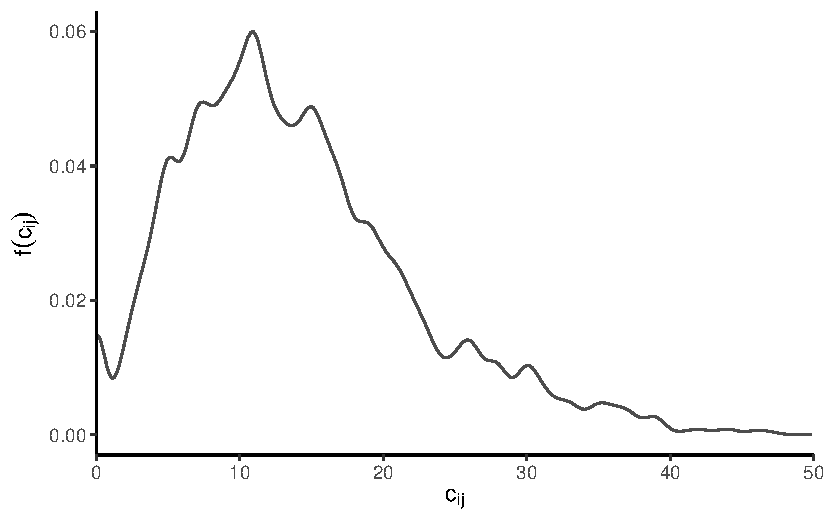
\includegraphics{tools-report_files/figure-pdf/fig-TLD-empirical-1.pdf}

}

\caption{\label{fig-TLD-empirical}Trip length distribution of home to
full-time work trips (in estimated minutes by car) for the City of
Hamilton.}

\end{figure}

In our example, the y-axis \(f(c_{ij})\) is the probability density of a
trip at a given travel cost in minutes of travel \(c_{ij}\). It can be
observed that the probability density of a trip is highest when travel
time is around 11 minutes. It can also be seen that beyond the 30 min
mark approximately, the rate of probability density drastically
decreases. So, the probability of a trip of length 0 to 30 mins
occurring is 95\% (the area under the curve between these two x-value
points is 0.95). Trips outside of this range make up the remaining
probability.

Now we fit the parameters of the uniform, exponential, and gamma
functions (Equation~\ref{eq-uniform-imped}, Equation~\ref{eq-exp-imped},
Equation~\ref{eq-gamma-imped}) as closely to the TLD captured in
Figure~\ref{fig-TLD-empirical}. The R package
\href{https://cloud.r-project.org/web/packages/fitdistrplus/index.html}{\{fitdistrplus\}}
was used to generate parameters that best fit the TLD. The moment
matching estimation (MME) fitting method and the Nelder-Mead direct
optimization algorithm are used (Delignette-Muller and Dutang 2015). The
default values for the parameters of the three functions are summarised:

\begin{itemize}
\item
  \(f(c_{ij})^{uniform}\): \(T_{min}\) and \(T_{max}\) is 0 and 29 mins,
  respectively.
\item
  \(f(c_{ij})^{exponential}\): \(\beta\) (rate) is 0.07
\item
  \(f(c_{ij})^{gamma}\): \(\alpha\) (shape) is 3 and \(\sigma\) (rate)
  is 0.2
\end{itemize}

\begin{figure}

{\centering 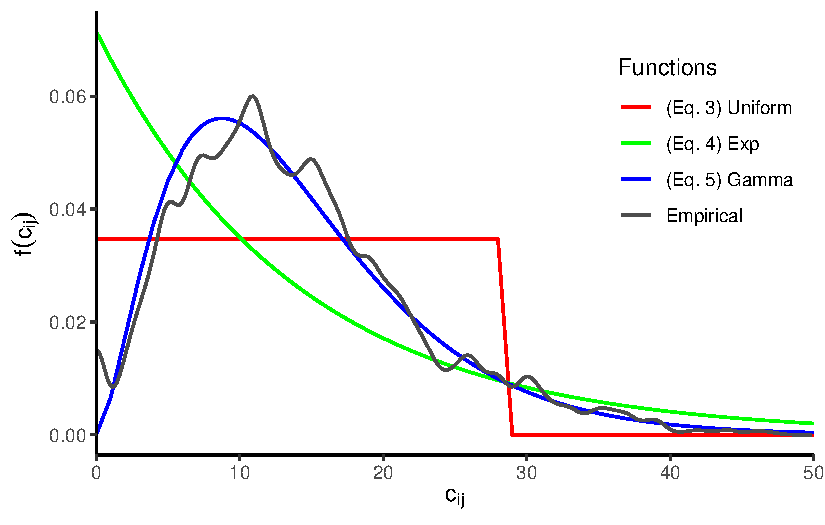
\includegraphics{tools-report_files/figure-pdf/fig-TLD-all-1.pdf}

}

\caption{\label{fig-TLD-all}Trip length distribution (empirical) with
fitted theoretical PDFs (coloured) of home to full-time work trips for
the City of Hamilton.}

\end{figure}

For curves shown in Figure~\ref{fig-TLD-all}: the higher the
\(f(c_{ij})\), the higher the probability density of travelling to reach
the opportunities at the destination.\footnote{Using \{fitdistrplus\},
  the parameters in all theoretical functions were selected through an
  optimization algorithm that minimizes the differences between all
  possible parameter range(s) and the empirical function for each
  theoretical function.}

The uniform impedance function (red), when implemented into an
accessibility calculation, would assume that the population is
indifferent to \emph{changes} in travel cost. The population at an
origin is assumed to either totally interact with an opportunity (if
it's a trip between 0 to 29 minutes - the \(T\) thresholds) or not
interact at all.

If the exponential (green) or gamma curve (blue) was implemented in an
accessibility calculation, then the analyst is assuming the population
is much more sensitive to changes in travel cost. However, the
exponential and gamma functions are quite a different shape, so they
depict a different response to the probability of traveling given a
travel cost \(c_{ij}\).

The exponential curve (green) is more intuitive to understand: the
shorter the travel cost \(c_{ij}\), the higher the \(f(c_{ij})\) value.
However, when compared to the empirical curve (black) (i.e., the
observed travel behaviour), we can see they do not closely match. Trip
lengths that are 11 mins in length have the highest probability density
of occurring and trips that are longer and shorter than this length
occur less often and are assigned decreasing \(f(c_{ij})\) values. For
these reasons, the gamma function (blue) provides a fit that is closest
to the empirical curve at the cost of a more complex mathematical
formulation.

The impedance function reflects significant assumptions about travel
behaviour. The selection of the type of function and associated
parameters reflects the impedance that populations face reaching
opportunities. How the impedance function is used to explain
accessibility will be discussed in Part II.

Again, feel free to explore the parameters interactively for the
uniform, exponential and gamma distributions using the interactive Shiny
R Application
\href{https://soukhova.shinyapps.io/Impedance-explained-shiny-app/}{here}.

\emph{The TLD used in this section is a subset of data from
\{TTS2016R\}, the goodness-of-fit criteria and diagnostics from
\{fitdistrplus\} are used for model parameter selection, plots are
generated using \{ggplot2\}, and spatial objects are manipulated using
\{sf\}, along with base \{R\} functions. View all the code and text
(including the interactive plot) in this
\href{https://github.com/soukhova/MJ-Accessibility-Blogs}{GitHub
repository}.}

\newpage

\hypertarget{sec-partII}{%
\section{Part II: Unconstrained and constrained
accessibility}\label{sec-partII}}

Within the context of transportation planning, accessibility (or
potential access) can be defined as a measure of the amount of
interaction a ``population'' at an origin potentially has with
``opportunities'' at destinations in a given region. It is a product of
the land-use and the population's means of transportation.

In this section, we distinguish between two types of accessibility
measures: \emph{unconstrained} and \emph{constrained} measures. The
distinction is important to help accessibility analysts to more clearly
interpret outputs.

First, we detail \textbf{unconstrained} accessibility. The general form
of the unconstrained measure, let's call it \(S_i\), is the measure
proposed by (Hansen 1959). Many accessibility measures are derived and
continue to be derived from this proposed formulation. \(S_i\) is an
accessibility value that is calculated for each spatial unit, and is
appropriately termed \emph{location-based accessibility}. This value is
the summation of all the \(O_j\) available (i.e., reachable) at each
spatial unit according to some impedance function \(f(c_{ij})\). \(S_i\)
is defined in Equation~\ref{eq-hansen-access-2}:

\begin{equation}\protect\hypertarget{eq-hansen-access-2}{}{
S_i = \sum_{j=1}^JO_j \cdot f(c_{ij})
}\label{eq-hansen-access-2}\end{equation}

\noindent Where:

\begin{itemize}
\tightlist
\item
  \(c_{ij}\) is a measure of the cost of moving between \(i\) and \(j\).
\item
  \(f(\cdot)\) is an impedance function of \(c_{ij}\); it can take the
  form of any monotonically decreasing function chosen based on positive
  or normative criteria (Paez, Scott, and Morency 2012).
\item
  \(i\) is a set of origin locations in the region (\(i = 1,\cdots,N\)).
\item
  \(j\) is a set of destination locations in the
  region(\(j = 1,\cdots,J\)).
\item
  \(O_j\) is the number of opportunities at location \(j\);
  \(O = \sum_{j=1}^J O_j\) is the total supply of opportunities in the
  study region.
\end{itemize}

Many variations of \(S_i\) have been proposed - but largely they focus
on tweaks to the type of \(f(c_{ij})\) used. This measure counts \(O_j\)
(after being weighted by \(f(c_{ij})\)) for each \(i\). This means that
the score assigned to each \(i\) is the summation of all the
opportunities that can \emph{potentially} be interacted with.

In lay terms, \(S_i\) is a measure of the number of opportunities that
someone at \(i\) can potentially interact with, given their travel
behaviour. However, counting all opportunities of potential interaction
may not suit certain opportunities. Consider the following hypothetical
example.

One can live in a part of the city where they have relatively high
accessibility \(S_i\) to jobs as a result of land-use (e.g., close to a
commercial business district) and transportation options (e.g., great
roads, excellent transit). Say \(S_i\) is a value of ``10,000 potential
job opportunities'' for a neighbourhood \(i\). Now, imagine if their
adjacent neighbourhoods have 15,000 people who can also reach those same
10,000 job opportunities. Though they can potentially interact with a
\emph{relatively} high \(S_i\) value of 10,000 opportunities, they may
have less \emph{available} opportunities as a result of relatively high
neighbouring demand for opportunities. When compared to other areas of
the city with relatively lower \(S_i\) values but with a similar level
of job opportunities and population demand, those other areas in the
city may have more potential \emph{spatial availability} than the
neighbourhood where our hypothetical person lives.

This concept is formally known as \emph{competition}, and has been
applied within the influential accessibility works of Shen (1998) and
Weibull (1976) as well as the widely used floating catchment areas
methods (e.g., the two step floating catchment area (2SFCA) approach of
Luo and Wang (2003)). We can think of these works as adjustments to
\(S_i\) (unconstrained accessibility) that account for the population's
demand for opportunities in the region of interest.

In a recently published journal article, an alternative derivation of
competitive accessibility that \emph{constrains} the results to match
known quantities in the system is proposed (Soukhov et al. 2023). These
known quantities can be the total number of opportunities or the total
population in the region under analysis. Since we constrain one of those
two (opportunities or population), we think of this measure as a
\emph{singly-constrained} competitive accessibility measure (\(V_i\)).

In \(V_i\), the total number of opportunities in the study region are
preserved. So if a urban region has 100,000 opportunities, at the end of
the analysis, the sum of \emph{all} \(V_i\) values in the region is
100,000. How is this achieved? As a result of the proportional
allocation feature: opportunities are allocated proportionally to each
spatial units in the region based on the relative travel impedance and
relative population density. We call this measure \emph{spatial
availability} which we denote as \(V_i\) to distinguish it from
unconstrained accessibility \(S_i\). Spatial availability and its
mathematical formulation is defined in Equation~\ref{eq-spatial-avail}:

\begin{equation}\protect\hypertarget{eq-spatial-avail}{}{
\begin{array}{l}
\\V_{i} = \sum_{j=1}^NO_jF^t_{ij} \\
\text{Where: } F^t_{ij} = \frac{F^p_{i} \cdot F^c_{ij}}{\sum_{i=1}^N F^p_{i} \cdot
F^c_{ij}}
\end{array}
}\label{eq-spatial-avail}\end{equation}

\noindent Where \(V_i\) contains the opportunities, just as in the
\emph{unconstrained} accessibility measure \(S_i\), but the allocation
depends on balancing factor \(F^t_{ij}\). The sum of of \(F^t_{ij}\) in
the region adds up to 1, which is how the sum of the spatial
availability is equal to the sum of \(O_j\). Revising our hypothetical
example of a urban region with 100,000 opportunities: it can be
understood that both measures (\(S_i\) and \(V_i\)) are weighted sums of
opportunities, but in \(S_i\) the sum of all opportunities may be more
or less than the 100,000. In contrast, thanks to the proportional
allocation balancing factors in \(V_i\), the sum of \(V_i\) values
across the region is constrained to equal 100,00 opportunities.

For additional context, within \(V_i\):

\begin{itemize}
\tightlist
\item
  \(F^t_{ij}\) is a balancing factor defined the population balancing
  factor (\(F^p_{i} = \frac{P_{i}}{\sum_{i=1}^N P_{i}}\)) and travel
  impedance balancing factor
  (\(F^c_{ij} = \frac{f(c_{ij})}{\sum_{i=1}^N f(c_{ij})}\))
\end{itemize}

The balancing factor \(F^p_{i}\) corresponds to the proportion of the
population in origin \(i\) relative to the population in the region. On
the right hand side of the equation, the numerator \(P_{i}\) is the
population in neighbourhood \(i\). The summation in the denominator is
over \(i=1,\cdots,N\), and adds up to the total population of the region
under analysis. What does this mean practically? It means,
neighbourhoods with a higher density of people get allocated more
opportunities (i.e., a larger \(F^p_{i}\) value), and less population
dense neighborhoods get allocated smaller amounts. This measure is
sensitive to demand: more people who are seeking opportunities get
allocated more opportunities.

The second balancing factor, \(F^c_{ij}\) is the travel impedance
balancing factor. It uses the impedance function (i.e., probability of
travel given travel costs) to proportionally allocate more opportunities
to neighbourhoods that are closer to (or contain) a higher density of
opportunities. That is, this balancing factor assumes that populations
within neighbourhoods that have lower travel impedance (less costly
travel) to opportunities are \emph{more willing} to take these
opportunities, resulting in a higher value of \(F^c_{ij}\) for the
neighbourhood. Indeed, the travel cost balancing factor can be thought
of as the proportion of the population at an `origin' neighbourhood
\(i\) willing to travel to a `destination' neighbourhood \(j\),
conditional on the travel behavior as described by the impedance
function. What does this mean practically? It means, the higher the
\(F^c_{ij}\) for a neighbourhood, the more opportunities get allocated
to this neighbourhood than other neighbourhoods.

Overall, \(S_i\) and \(V_i\) can be complex to understand - but the
outputs may clarify their intuition.

\newpage

\hypertarget{differences-in-unconstrained-and-constrained-accessibility}{%
\subsection{Differences in unconstrained and constrained
accessibility}\label{differences-in-unconstrained-and-constrained-accessibility}}

For this demonstration, \textbf{unconstrained} and \textbf{constrained}
accessibility are calculated using data taken from the R data package
\{TTS0216R\}. This package contains a subset of home to work (full-time)
flows from the 2016 Transportation Tomorrow Survey (TTS) as well as
travel time by car calculated using \{r5r\}. \{TTS2016R\} is detailed in
this publication (Soukhov and Páez 2023) and is freely available to be
explored \href{https://soukhova.github.io/TTS2016R/}{here}. The focus of
this demonstration is the City of Hamilton, Canada, a city approximately
70 km south-west of Toronto, and within the TTS survey area.

A calibrated gamma distribution probability density function serves as
the impedance function for the analysis and is shown in
Figure~\ref{fig-gamma} (\(\alpha\) (shape) is 3 and \(\sigma\) (rate) is
0.2). The data set and parameters were fit using the empirical data and
discussed in Part I. As a refresher, a gamma distribution form was
selected as it best fits the sample of home to full-time work trips
beginning and ending in the City of Hamilton. The values along the
y-axis can be interpreted as the probability density of a trip at a
certain travel time \(c_{ij}\) of occurring i.e., trips of length 9
minutes are the most likely to occur and hence are assigned the highest
relative \(f(c_{ij})\) value.

\begin{figure}

{\centering 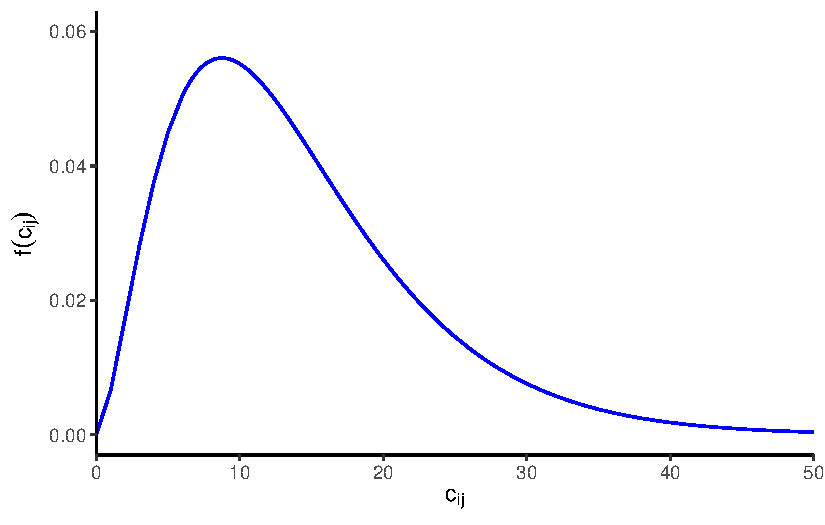
\includegraphics{tools-report_files/figure-pdf/fig-gamma-1.pdf}

}

\caption{\label{fig-gamma}The fitted theoretical gamma distribution
travel impedance function of home-to-work trips (in estimated minutes by
car) for the City of Hamilton.}

\end{figure}

The \{accessibility\} package is used to conveniently calculate
unconstrained accessibility \(S_i\) (Equation~\ref{eq-hansen-access-2})
and singly-constrained competitive accessibility \(V_i\)
(Equation~\ref{eq-spatial-avail}). The resulting \(S_i\) (Purples) and
\(V_i\) (Greens) are shown in
Figure~\ref{fig-raw-con-and-unconstrained-access}. Both measures reflect
\emph{potential interaction} with jobs based on empirical home-to-work
travel behaviour in Hamilton: people who reside in each spatial unit
make certain trips to other spatial units (in Hamilton) and these trips
have a certain travel time (travel cost \(c_ij\)) with associated gamma
impedance \(f(c_{ij}\) value. These observed trip patterns inform the
calculated \(S_i\) and \(V_i\) values for each spatial unit. What's
notable is the difference in the \textbf{magnitude} and the
\textbf{interpretation} of unconstrained (\(S_i\)) and constrained
(\(V_i\)) values.

\begin{figure}

{\centering 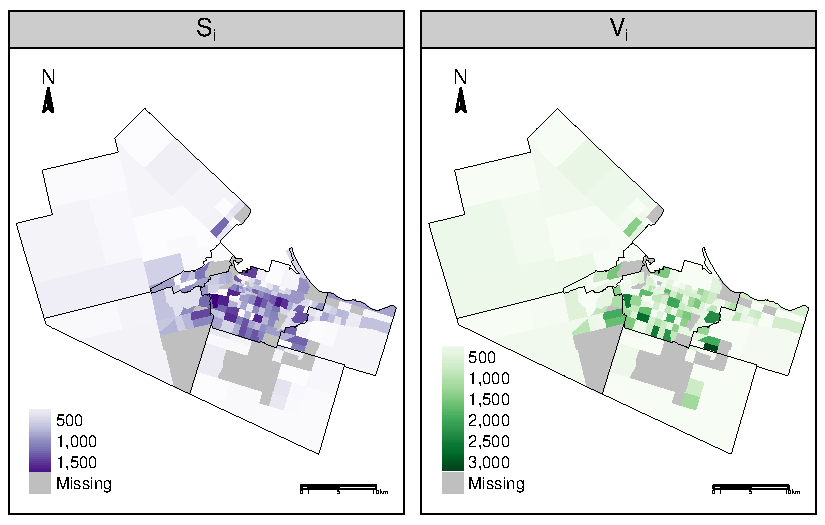
\includegraphics{tools-report_files/figure-pdf/fig-raw-con-and-unconstrained-access-1.pdf}

}

\caption{\label{fig-raw-con-and-unconstrained-access}The unconstrained
(Si) and constrained (Vi) accessibility (a.k.a. spatial availability)
scores for the City of Hamilton. Calculated using an empirically
calibrated gamma distribution travel impedance function.}

\end{figure}

Looking at the left plot \(S_i\) in
Figure~\ref{fig-raw-con-and-unconstrained-access}, the values reflect
the sum of jobs that can be potentially interacted with by the
population at each \(i\) multiplied by their probability of being
reached as informed by the calculated travel impedance \(f(c_{ij})\)
value. The maximum \(S_i\) value is the darkest purple, and that value
means that people who reside in those spatial units have the
\emph{lowest} travel impedance and \emph{highest} concentration of
potential job interaction for the region. The value itself does not have
a specific meaning as it is just the sum of `weighted' jobs: it can be
interpreted as a relative score of potential interaction based on the
observed trip patterns of people who reside in the City. For instance,
areas within the centre of Hamilton have the highest values, this is
both where jobs are largely clustered as well as major roadways
(highways are pictured) and denser street networks.

Now looking at the right plot \(V_i\) (constrained) in
Figure~\ref{fig-raw-con-and-unconstrained-access}, the values reflect
the sum of the proportionally allocated (based on travel impedance and
population) \emph{potential job interactions}. In other words, each
value of \(V_i\) is the number of jobs that the spatial unit \(i\) can
interact with based on the observed trips made from that spatial unit's
impedance values relative to how others in the region can interact with
the jobs. Unlike \(S_i\), the raw values of \(V_i\) do have a meaning in
addition to being a relative score of \emph{competitive} potential job
interactions. This score reflects the potential \emph{availability} of
jobs: potential job interactions are less likely to occur if the
concentration of jobs is low and the density of people interacting with
those jobs are high. So as we can observe in the plot, \(V_i\) considers
population demand, and as the centre of Hamilton is the most densely
populated area in the city, the centre does not share the same intensity
of trend as \(S_i\).

The \(V_i\) value in itself is also meaningful. \(V_i\) values
communicates the number of potentially \emph{available} job interactions
per each spatial unit \(i\) out of all the jobs in the region. If all
\(V_i\) values are added together, the sum equals 108,526 - the total
number of jobs taken by people who live and work (full-time) within the
City from the data set. So in the most green spatial unit, 3,160
potentially available job interactions can occur out of the total
108,526 jobs. Again, \(V_i\) is produced through proportional
allocation, the total number of jobs is divided up and assigned to each
spatial unit based on the impedance to reach jobs and the population who
also interact with these potential opportunities.

To more equally compare \(S_i\) and \(V_i\) and make sense of the
`highs' and `lows', it may be useful to standardise the values onto a
similar scale. In Figure~\ref{fig-perc-con-and-unconstrained-access},
the values as presented as a percentage of the regional sum (i.e., a \%
of the sum of all \(S_i\) values and the \% of the sum of all \(V_i\)
values) are visualized for the centre of Hamilton.

\begin{figure}

{\centering 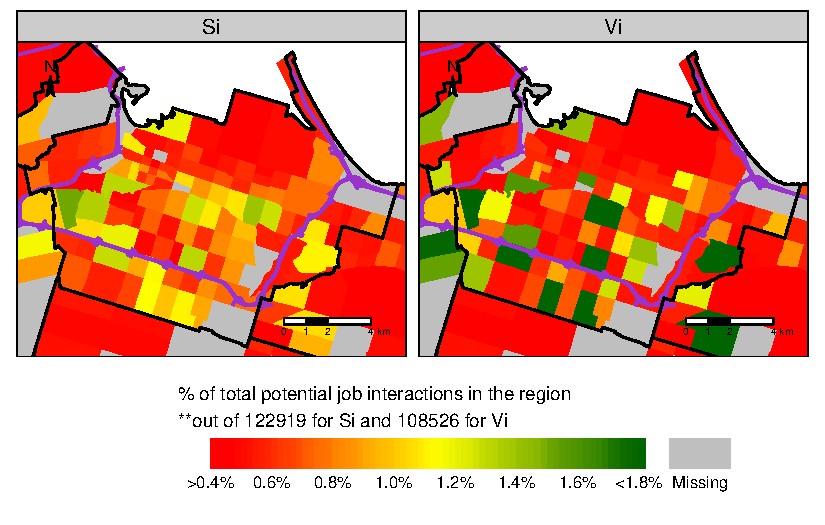
\includegraphics{tools-report_files/figure-pdf/fig-perc-con-and-unconstrained-access-1.pdf}

}

\caption{\label{fig-perc-con-and-unconstrained-access}Scaled
unconstrained (Si) and constrained (Vi) accessibility scores for
Hamilton Centre. Values are presented as a percentage of the total sum
of scores within the City of Hamilton. Major highways are shown in
purple for spatial reference. Values are calculated using an empirically
calibrated gamma distribution travel impedance function.}

\end{figure}

Examining \(S_i\) (left plot) in
Figure~\ref{fig-perc-con-and-unconstrained-access}: unconstrained
accessibility. Neighbourhoods with `high' accessibility (e.g., greens,
that start at 1.3\% relative values or higher) can potentially interact
with 1417 jobs or more as informed by observed travel behaviour. These
raw values are difficult to interpret, so seeing a neighbourhood as
being an area of relative `high', `medium' (yellows) or `low' (reds)
accessibility value simplifies the interpretation of `potential
interaction' with jobs; as long as we ignore \emph{competition}.

Examining the plot on the right side in
Figure~\ref{fig-perc-con-and-unconstrained-access}, visuals \(V_i\)
spatial availability. This measure does not ignore competition for
potential job interaction. The general trend between both plots are
similar, but a handful of spatial units that are more intensely green or
red/orange can be seen. These differences are a result of competition.
Within this region, spatial units that are more densely populated as
well as having below average travel impedance have higher standardized
\(V_i\) values than \(S_i\) values. Conversely, below average population
and above average travel impedance yields spatial availability \(V_i\)
values that are lower than \(S_i\).

In essence, \(V_i\) reflects travel impedance like \(S_i\) does, but it
also considers competition. Spatial units with orange/green \(S_i\) that
have red \(V_i\) are a cause for concern: they likely have low travel
impedance but high competition that makes their \(V_i\) relatively low.
Conversely, spatial units with orange/red \(S_i\) that have green
\(V_i\) have high travel impedance but low competition for their
opportunities so their spatial availability of jobs may in fact be
alright. Spatial availability adds an additional layer of consideration
into the accessibility measure, and as such, reveals more about the
region (under the travel behaviour and opportunity accessed
assumptions).

Across both \(S_i\) and \(V_i\) in
Figure~\ref{fig-perc-con-and-unconstrained-access}, we can see some
common low values (red) located in the north end of the city. From
unconstrained accessibility, we know these TAZ have high relative travel
impedance - this may be because people who work in the north end do not
live relatively close to these opportunities so have high relative
travel times. Interestingly though, we can confirm that there is a high
relative number of jobs within these TAZ (see
Figure~\ref{fig-worker-job-plot} below), however, even the number of
jobs does not balance the impedance value and higher demand for those
jobs. Hence, the constrained accessibility measure is also low.

\begin{figure}

{\centering 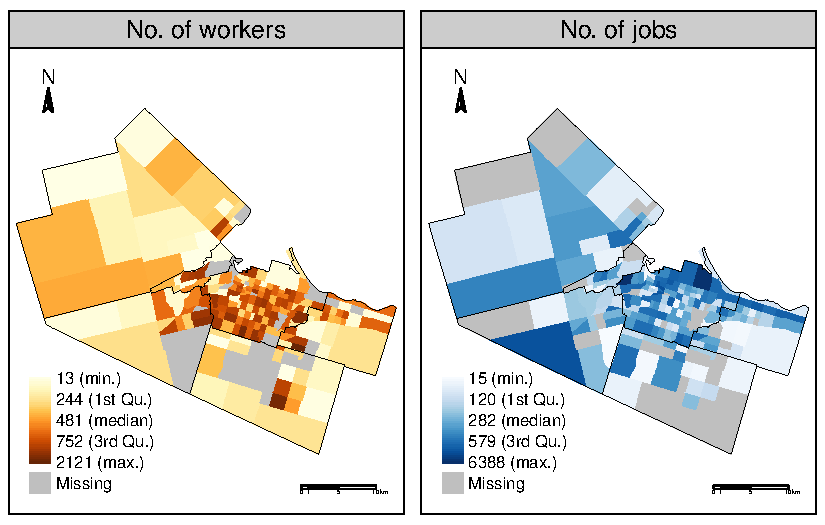
\includegraphics{tools-report_files/figure-pdf/fig-worker-job-plot-1.pdf}

}

\caption{\label{fig-worker-job-plot}The number of workers and jobs in
Hamilton Center. Note: only workers who reside and work within Hamilton
Center are considered in the accessibility calculations for this
demonstration.}

\end{figure}

\hypertarget{concluding-remarks}{%
\subsection{Concluding remarks}\label{concluding-remarks}}

Accessibility is a unique measure that characterises the relationship
between land-use (where populations reside and the opportunities they
can interact with) in addition to transportation travel impedance. How
the relationship is conceptualization (i.e., if there's competition or
not) and how the travel impedance is calibrated (i.e., what function
describes travel behaviour) are critical in determining what the final
values are and how to interpret them.

In this section, we outlined two branches of accessibility measures:
unconstrained (\(S_i\) in this case) and constrained (spatial
availability \(V_i\)). Unconstrained accessibility only considers
opportunities that could be interacted with while constrained considers
\emph{both} those opportunities and the demand for those opportunities
in addition to having that property of proportional allocation. This
property allows the raw values of \(V_i\) to be interpreted without any
sort of transformation or standardizing; \(V_i\) is simply the number of
opportunities that can be potentially interacted with out of \emph{all}
opportunities in the region.

\(V_i\) provides insights that \(S_i\) does not. Firstly, it considers
considers competition from demand. Secondly, it does not need to be
standardized to be understood. These two insights are important:

\begin{itemize}
\tightlist
\item
  \textbf{Considering competition}: places of employment are a
  \emph{non-divisible} type of opportunity, they only allow one person
  to take one job. Unless there's a reason to \emph{not} consider
  competition, measuring access to opportunities that have some capacity
  using an unconstrained measure \(S_i\) does not make much theoretical
  sense; this will be explored in subsequent report(s).
\item
  \textbf{Interpretation}: a spatial unit has a certain number of
  \(V_i\), opportunities that are spatially available for interaction.
  We can tangibly interpret if that's high or low (out of the total
  number of opportunities). Further, we can also divide \(V_i\) by
  population at that origin to obtain opportunity per capita values.
  This value can be used as a benchmark to compare opportunity per
  capita or levels of service across areas of the region, between
  regions, and/or across time; again, this will be explored in
  subsequent report(s).
\end{itemize}

Ultimately, unconstrained accessibility \(S_i\) tells you how many
opportunities can be potentially reached. Spatial availability \(V_i\)
tells you how many opportunities are \emph{available} based on how many
can be potentially reached and demanded.

Accessibility analysis sheds light on regions of inequitable potential
access. Assumptions on what region to analyse, what population and
opportunities are the subject of analysis, the travel cost unit and
calculation, the impedance function and the measure used all impact the
final results. But ultimately, the output represents the number of
opportunities that could \emph{potentially} be reached from each origin.
It is critical that the assumptions embedded within each step of
analysis are understood so that the final value can be interpreted and
inequities be identified.

Once these spatial inequities have been identified - what do we do about
it? That is the subject for future sections.

Openness is legitimacy: this report was written in a R environment and
can be fully reproduced from the materials available at this GitHub
(\href{https://github.com/soukhova/MJ-Accessibility-Blogs}{repository}).
If interested, see the open access PDF of the full article (which
includes the mathematical formulation for the spatial availability
function) in the references (Soukhov et al. 2023).

\emph{The data used in this section is a subset of data from
\{TTS2016R\}, the plots are created using \{tmap\}, and spatial objects
are manipulated using \{sf\}, along with base \{R\} functions.}

\newpage

\hypertarget{references}{%
\section{References}\label{references}}

\hypertarget{refs}{}
\begin{CSLReferences}{1}{0}
\leavevmode\vadjust pre{\hypertarget{ref-Muller2016}{}}%
Delignette-Muller, Marie Laure, and Christophe Dutang. 2015.
{``{fitdistrplus}: An {R} Package for Fitting Distributions.''}
\emph{Journal of Statistical Software} 64 (4): 1--34.
\url{https://doi.org/10.18637/jss.v064.i04}.

\leavevmode\vadjust pre{\hypertarget{ref-hansen1959}{}}%
Hansen, Walter G. 1959. {``How Accessibility Shapes Land Use.''}
\emph{Journal of the American Institute of Planners} 25 (2): 73--76.
\url{https://doi.org/10.1080/01944365908978307}.

\leavevmode\vadjust pre{\hypertarget{ref-luo2003}{}}%
Luo, Wei, and Fahui Wang. 2003. {``Measures of Spatial Accessibility to
Health Care in a GIS Environment: Synthesis and a Case Study in the
Chicago Region.''} \emph{Environment and Planning B: Planning and
Design} 30 (6): 865--84. \url{https://doi.org/10.1068/b29120}.

\leavevmode\vadjust pre{\hypertarget{ref-paez2012measuring}{}}%
Paez, A., D. M. Scott, and C. Morency. 2012. {``Measuring Accessibility:
Positive and Normative Implementations of Various Accessibility
Indicators.''} Journal Article. \emph{Journal of Transport Geography}
25: 141--53. \url{https://doi.org/10.1016/j.jtrangeo.2012.03.016}.

\leavevmode\vadjust pre{\hypertarget{ref-shen1998}{}}%
Shen, Q. 1998. {``Location Characteristics of Inner-City Neighborhoods
and Employment Accessibility of Low-Wage Workers.''} \emph{Environment
and Planning B: Planning and Design} 25 (3): 345--65.
\url{https://doi.org/10.1068/b250345}.

\leavevmode\vadjust pre{\hypertarget{ref-soukhovIntroducingSpatialAvailability2023}{}}%
Soukhov, Anastasia, Antonio Paez, Christopher D. Higgins, and Moataz
Mohamed. 2023. {``Introducing Spatial Availability, a Singly-Constrained
Measure of Competitive Accessibility \textbar{} {PLOS ONE}.''}
\emph{PLOS ONE}, 1--30.
https://doi.org/\href{https://\%20doi.org/10.1371/journal.pone.0278468}{https://
doi.org/10.1371/journal.pone.0278468}.

\leavevmode\vadjust pre{\hypertarget{ref-soukhovTTS2016RDataSet2023}{}}%
Soukhov, Anastasia, and Antonio Páez. 2023. {``{TTS2016R}: {A} Data Set
to Study Population and Employment Patterns from the 2016
{Transportation Tomorrow Survey} in the {Greater Golden Horseshoe} Area,
{Ontario}, {Canada}.''} \emph{Environment and Planning B: Urban
Analytics and City Science}, January, 23998083221146781.
\url{https://doi.org/10.1177/23998083221146781}.

\leavevmode\vadjust pre{\hypertarget{ref-weibull_axiomatic_1976}{}}%
Weibull, Jörgen W. 1976. {``An Axiomatic Approach to the Measurement of
Accessibility.''} \emph{Regional Science and Urban Economics} 6 (4):
357--79. \url{https://doi.org/10.1016/0166-0462(76)90031-4}.

\end{CSLReferences}

\newpage

% LAST PAGE
% This page is left blank on purpose

% Set style for this page
\thispagestyle{empty}

% Council logo at bottom
\begin{center}
    \begin{figure}[b]
        
\includegraphics[width=\textwidth]{images/sshrc-canada-banner.png}
    \end{figure}    
\end{center}



\end{document}
